\documentclass[aspectratio=169,11pt]{beamer}

\usepackage[T1]{fontenc}
\usepackage{lmodern}
\usepackage{booktabs}
\usepackage{tabularx}
\usepackage{tikz}
\usetikzlibrary{arrows.meta,positioning}
\usepackage{xcolor}
\usepackage{hyperref}

\definecolor{navy}{HTML}{172554}
\definecolor{teal}{HTML}{4F46E5}
\definecolor{green}{HTML}{059669}
\definecolor{orange}{HTML}{F97316}
\definecolor{cyan}{HTML}{0891B2}
\definecolor{slate}{HTML}{334155}
\definecolor{lightblue}{HTML}{EEF2FF}
\definecolor{lightgrey}{HTML}{F8FAFC}
\definecolor{lightcyan}{HTML}{ECFEFF}

\usetheme{default}
\setbeamercolor{normal text}{fg=slate,bg=lightgrey}
\setbeamercolor{background canvas}{bg=lightgrey}
\setbeamercolor{structure}{fg=teal}
\setbeamercolor{frametitle}{fg=white,bg=navy}
\setbeamercolor{title}{fg=navy}
\setbeamercolor{block title}{bg=teal,fg=white}
\setbeamercolor{block body}{bg=lightblue,fg=black}
\setbeamercolor{block title alerted}{bg=orange,fg=white}
\setbeamercolor{block body alerted}{bg=orange!10,fg=slate}
\setbeamercolor{itemize item}{fg=teal}
\setbeamercolor{itemize subitem}{fg=cyan}
\setbeamercolor{enumerate item}{fg=teal}
\setbeamertemplate{blocks}[rounded][shadow=true]
\setbeamertemplate{itemize item}{\raise0.15ex\hbox{\scriptsize$\blacktriangleright$}}
\setbeamertemplate{itemize subitem}{\raise0.1ex\hbox{\tiny$\bullet$}}
\setbeamertemplate{navigation symbols}{}
\setbeamertemplate{footline}{}
\setbeamertemplate{frametitle}{
  \nointerlineskip
  \begin{beamercolorbox}[wd=\paperwidth,ht=3.2ex,dp=1.1ex,leftskip=0.7cm]{frametitle}
    \usebeamerfont{frametitle}\insertframetitle
  \end{beamercolorbox}
}

\newcommand{\source}[2]{\href{#1}{\textcolor{teal}{#2}}}

\title{From Open Data to Safer Travel Decisions}
\subtitle{Open Data contribution to the onboarding presentation}
\author{Team member: \underline{\hspace{3.5cm}}}
\date{August 2026}

\begin{document}

\begin{frame}{The five datasets we actually need}
  \scriptsize
  \renewcommand{\arraystretch}{1.18}
  \begin{tabularx}{\textwidth}{p{2.5cm}p{2.0cm}X p{2.1cm}p{1.5cm}}
    \toprule
    \textbf{Open dataset} & \textbf{Access / source refresh} &
    \textbf{Why it is needed} & \textbf{Our planned refresh} &
    \textbf{Licence} \\
    \midrule
    Past-hour pedestrian counts per minute &
    API/CSV; about every 15 min &
    Current pedestrian volume and high-crowd alerts &
    Every 15 min &
    CC BY 4.0 \\

    Pedestrian counts per hour (2009--present) &
    API/CSV; monthly &
    Sensor-specific baselines, quiet-time patterns and next-hour forecasts &
    Monthly &
    CC BY 4.0 \\

    Pedestrian sensor locations &
    API/CSV; maintained as needed &
    Coordinates, operating status, direction and relocation notes &
    Daily metadata check &
    CC BY 4.0 \\

    Landmarks and places of interest &
    API/CSV; periodic &
    Candidate parks, gardens, libraries and public facilities for a break &
    Once per iteration &
    CC BY 4.0 \\

    OpenStreetMap pedestrian network &
    OSM extracts/API; continuously edited &
    Walkable paths and connections needed to calculate candidate routes &
    Versioned iteration snapshot &
    ODbL 1.0 \\
    \bottomrule
  \end{tabularx}

  \vspace{0.25em}
  \textbf{Selection rule:} every source must support a user story; no dataset is
  included merely because it is available.

  % Speaker notes:
  % The first four sources are from the City of Melbourne. OpenStreetMap fills a
  % genuine gap: point-based sensor data cannot by itself produce a walking route.
  % Public-transport GTFS can be added in a later iteration if transport-stop
  % integration is accepted into scope.
\end{frame}

\begin{frame}{How each source creates customer value}
  \small
  \begin{columns}[T,onlytextwidth]
    \column{0.32\textwidth}
      \begin{block}{Hindsight\\What happened?}
        Historical hourly counts show:
        \begin{itemize}
          \item recurring peak periods;
          \item quieter weekday/time combinations;
          \item seasonal and location differences.
        \end{itemize}
        \textbf{User benefit:} plan travel for a historically quieter window.
      \end{block}

    \column{0.32\textwidth}
      \begin{block}{Insight\\What is happening?}
        Live counts joined to sensor locations show:
        \begin{itemize}
          \item current relative crowd level;
          \item monitored low-activity areas;
          \item nearby candidate refuge locations.
        \end{itemize}
        \textbf{User benefit:} avoid an unexpectedly crowded corridor.
      \end{block}

    \column{0.32\textwidth}
      \begin{block}{Foresight\\What may happen?}
        Recent counts compared with historical patterns provide:
        \begin{itemize}
          \item next-hour crowd estimate;
          \item confidence or uncertainty;
          \item an early rerouting prompt.
        \end{itemize}
        \textbf{User benefit:} adjust the journey before conditions worsen.
      \end{block}
  \end{columns}

  \vspace{0.25em}
  \begin{center}
    \textcolor{orange}{\textbf{Pedestrian volume is a sensory-load proxy, not a
    guarantee that a route or place is ``safe''.}}
  \end{center}
\end{frame}

\begin{frame}{Planned data pipeline and quality controls}
  \centering
  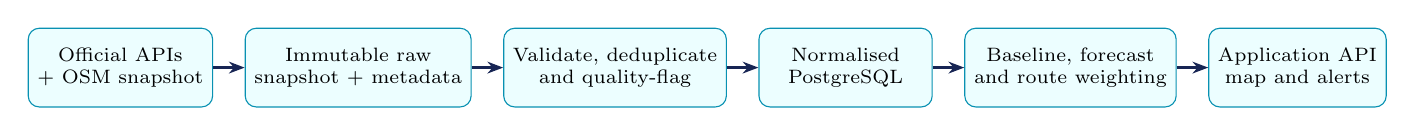
\begin{tikzpicture}[
      node distance=5mm and 4mm,
      box/.style={
        draw=cyan, rounded corners, fill=lightcyan, align=center,
        minimum width=2.2cm, minimum height=1.0cm, font=\scriptsize
      },
      arrow/.style={-{Stealth[length=2mm]}, thick, draw=navy}
    ]
    \node[box] (source) {Official APIs\\+ OSM snapshot};
    \node[box, right=of source] (raw) {Immutable raw\\snapshot + metadata};
    \node[box, right=of raw] (quality) {Validate, deduplicate\\and quality-flag};
    \node[box, right=of quality] (db) {Normalised\\PostgreSQL};
    \node[box, right=of db] (model) {Baseline, forecast\\and route weighting};
    \node[box, right=of model] (app) {Application API\\map and alerts};

    \draw[arrow] (source) -- (raw);
    \draw[arrow] (raw) -- (quality);
    \draw[arrow] (quality) -- (db);
    \draw[arrow] (db) -- (model);
    \draw[arrow] (model) -- (app);
  \end{tikzpicture}

  \vspace{0.8em}
  \begin{columns}[T,onlytextwidth]
    \column{0.49\textwidth}
      \begin{block}{Ingestion controls}
        \begin{itemize}
          \item Record source URL, retrieval time and licence.
          \item Validate IDs, timestamps, coordinates and non-negative counts.
          \item Upsert on \texttt{(sensor\_id, observed\_at)}.
          \item Quarantine invalid records; never silently discard them.
        \end{itemize}
      \end{block}

    \column{0.49\textwidth}
      \begin{block}{Interpretation controls}
        \begin{itemize}
          \item Distinguish zero movement from sensor/API failure.
          \item Preserve sensor relocation history and active periods.
          \item Display freshness, coverage and prediction confidence.
          \item Version raw snapshots, transformations and model outputs.
        \end{itemize}
      \end{block}
  \end{columns}
\end{frame}

\begin{frame}{Simple ERD: four ideas we store}
  \centering
  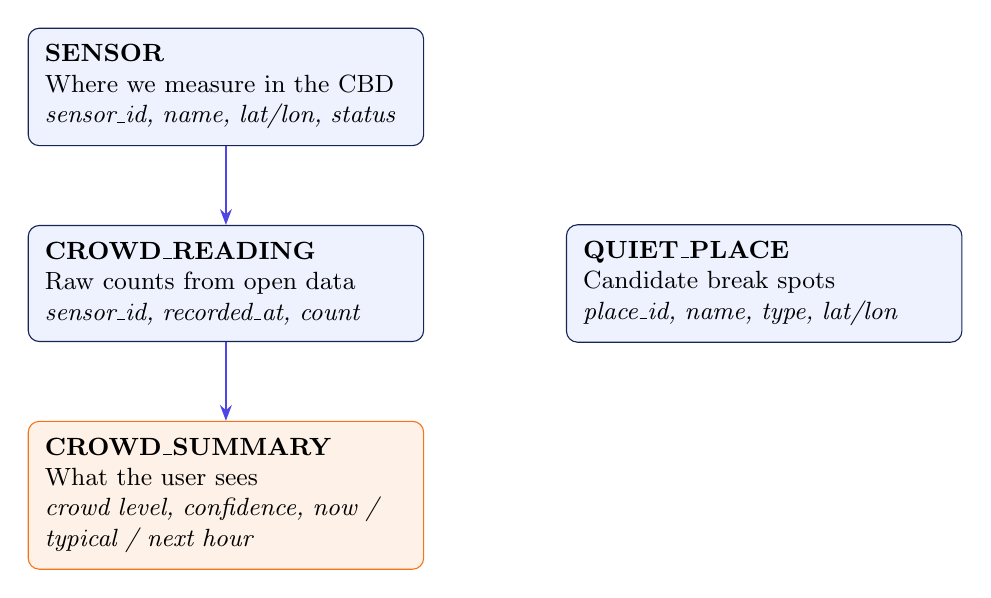
\begin{tikzpicture}[
      entity/.style={
        draw=navy, rounded corners, fill=lightblue, align=left,
        font=\small, text width=4.6cm, inner sep=6pt
      },
      derived/.style={
        draw=orange, rounded corners, fill=orange!10, align=left,
        font=\small, text width=4.6cm, inner sep=6pt
      },
      rel/.style={-{Stealth[length=2mm]}, thick, draw=teal},
      node distance=10mm
    ]
    \node[entity] (sensor) {
      \textbf{SENSOR}\\
      Where we measure in the CBD\\
      \textit{sensor\_id, name, lat/lon, status}
    };
    \node[entity, below=of sensor] (reading) {
      \textbf{CROWD\_READING}\\
      Raw counts from open data\\
      \textit{sensor\_id, recorded\_at, count}
    };
    \node[derived, below=of reading] (summary) {
      \textbf{CROWD\_SUMMARY}\\
      What the user sees\\
      \textit{crowd level, confidence, now / typical / next hour}
    };
    \node[entity, right=18mm of reading] (place) {
      \textbf{QUIET\_PLACE}\\
      Candidate break spots\\
      \textit{place\_id, name, type, lat/lon}
    };

    \draw[rel] (sensor) -- (reading);
    \draw[rel] (reading) -- (summary);
  \end{tikzpicture}

  \vspace{0.5em}
  \small
  \textbf{Explain in one line:} sensors collect readings; we turn readings into simple
  crowd summaries; quiet places are shown nearby on the map when needed.\\
  \textit{Walking routes (OpenStreetMap) sit in the app layer---omitted here to keep the model easy to explain.}
\end{frame}

\begin{frame}{Selected analytical approach: explainable first}
  \small
  \begin{columns}[T,onlytextwidth]
    \column{0.49\textwidth}
      \begin{block}{Crowd classification}
        Compare each observation with the same sensor's historical distribution
        for that weekday and hour:
        \begin{itemize}
          \item Low: at or below the 40th percentile;
          \item Moderate: 40th--75th percentile;
          \item High: above the 75th percentile.
        \end{itemize}
        This avoids one arbitrary threshold for differently sized locations.
      \end{block}

    \column{0.49\textwidth}
      \begin{block}{Next-hour forecast}
        Begin with an interpretable seasonal baseline:
        \begin{enumerate}
          \item historical median for sensor, weekday and hour;
          \item adjustment using the most recent observation;
          \item confidence based on sample size and data freshness;
          \item validate using MAE and high-crowd alert precision/recall.
        \end{enumerate}
      \end{block}
  \end{columns}

  \vspace{0.3em}
  \textbf{AI decision:} no opaque machine-learning model is required for
  onboarding. A more complex model should be adopted only if time-based
  validation proves that it improves forecasts without reducing explainability.

  \vspace{0.4em}
  \begin{alertblock}{Responsible interpretation}
    Use ``lower observed pedestrian activity'' and ``candidate refuge'', not
    ``sensory-safe''. Show stale-data warnings, geographic coverage gaps and
    uncertainty to prevent false reassurance.
  \end{alertblock}
\end{frame}

\begin{frame}{Data risks, mitigations and source links}
  \small
  \begin{tabularx}{\textwidth}{p{3.2cm}X}
    \toprule
    \textbf{Material risk} & \textbf{Planned mitigation} \\
    \midrule
    CBD sensors are not representative of every street &
    Show monitored coverage and do not extrapolate beyond defensible distance. \\
    Missing records have ambiguous meaning &
    Check sensor status and neighbouring readings; retain an
    unavailable/uncertain state rather than automatic interpolation. \\
    Events or construction break historical patterns &
    Lower forecast confidence and label these factors as outside current data
    coverage unless an approved source is added. \\
    A public facility may not be quiet or open &
    Treat it as a candidate and add validation/opening-hours evidence before
    recommending it as a refuge. \\
    Public data can still be stale or altered &
    Validate schema, retain checksummed snapshots and monitor last successful
    ingestion. \\
    \bottomrule
  \end{tabularx}

  \vspace{0.35em}
  \tiny
  \textbf{Official sources (accessed August 2026):}\\
  \source{https://data.melbourne.vic.gov.au/explore/dataset/pedestrian-counting-system-past-hour-counts-per-minute/}{Minute pedestrian counts}
  \quad
  \source{https://data.melbourne.vic.gov.au/explore/dataset/pedestrian-counting-system-monthly-counts-per-hour/}{Historical hourly counts}
  \quad
  \source{https://data.melbourne.vic.gov.au/explore/dataset/pedestrian-counting-system-sensor-locations/}{Sensor locations}\\
  \source{https://data.melbourne.vic.gov.au/explore/dataset/landmarks-and-places-of-interest-including-schools-theatres-health-services-spor/}{Landmarks and places of interest}
  \quad
  \source{https://www.openstreetmap.org/copyright}{OpenStreetMap copyright and ODbL}
  \quad
  \source{https://creativecommons.org/licenses/by/4.0/}{CC BY 4.0}

  % Speaker notes:
  % Close by emphasising traceability: every displayed recommendation should be
  % explainable through a source record, a documented transformation and a
  % versioned analytical rule.
\end{frame}

\end{document}
